\documentclass{beamer} \usetheme{Madrid}
\usecolortheme{beaver}

\usepackage[utf8]{inputenc}
\usepackage{mdframed}
\usepackage{minted}

\title{{\LaTeX} Workshop}
\subtitle{Fall 2020}

\author[]{Jack Leightcap\inst{1}\inst{2}}

\institute[IEEE, Wireless Club]{
    \inst{1}IEEE -- \url{nuieeeofficers@gmail.com}
    \and
    \inst{2}Wireless Club -- \url{nuwirelessclub@gmail.com}
}

\date[Fall 2020]{October 5, 2020}

\begin{document}
\frame{\titlepage}

\begin{frame}
    \frametitle{What is {\LaTeX}?}
    \vfill
    \begin{itemize}
        \item A plain-text method of document preparation and typesetting
        \item \emph{Compiled} into a document format (PDF, DVI, etc.)
        \item Started as an academic tool for mathematicians and computer scientists (Discrete, Algo!)
        \item Expansive set of packages on \texttt{CTAN}
    \end{itemize}
    \vfill
    \begin{center}
        \begin{figure}
        
\includegraphics[width={\columnwidth}/3]{logo.png}
        \caption{The {\LaTeX} Project Logo, CC BY 4.0}
    \end{figure}
    \end{center}
\end{frame}

\begin{frame}
    \frametitle{Comparison of {\LaTeX} to Graphical Editors}
    \begin{columns}[t]
        \begin{column}{{\textwidth}/2}
            \begin{center}
                \textbf{WYSIWYG}
            \end{center}
            \begin{itemize}
                \item ``Interpreted''
                \item Allows ambiguity
                \item More speed than control
                \item Platform-dependent
                \item Directly understood
                \item Combined composition and formatting
            \end{itemize}
        \end{column}
        \begin{column}{{\textwidth}/2}
            \begin{center}
                \textbf{WYSIWYT}
            \end{center}
            \begin{itemize}
                \item Compiled
                \item Unambiguous (pedantic)
                \item More control than speed
                \item Portable
                \item Layer of Abstraction
                \item Seperated composition and formatting
            \end{itemize}
        \end{column}
    \end{columns}
\end{frame}

\begin{frame}
    \vfill
    \centering\includegraphics[width=\textwidth]{Notes.png}
    \vfill
\end{frame}

\begin{frame}
    \vfill
    \centering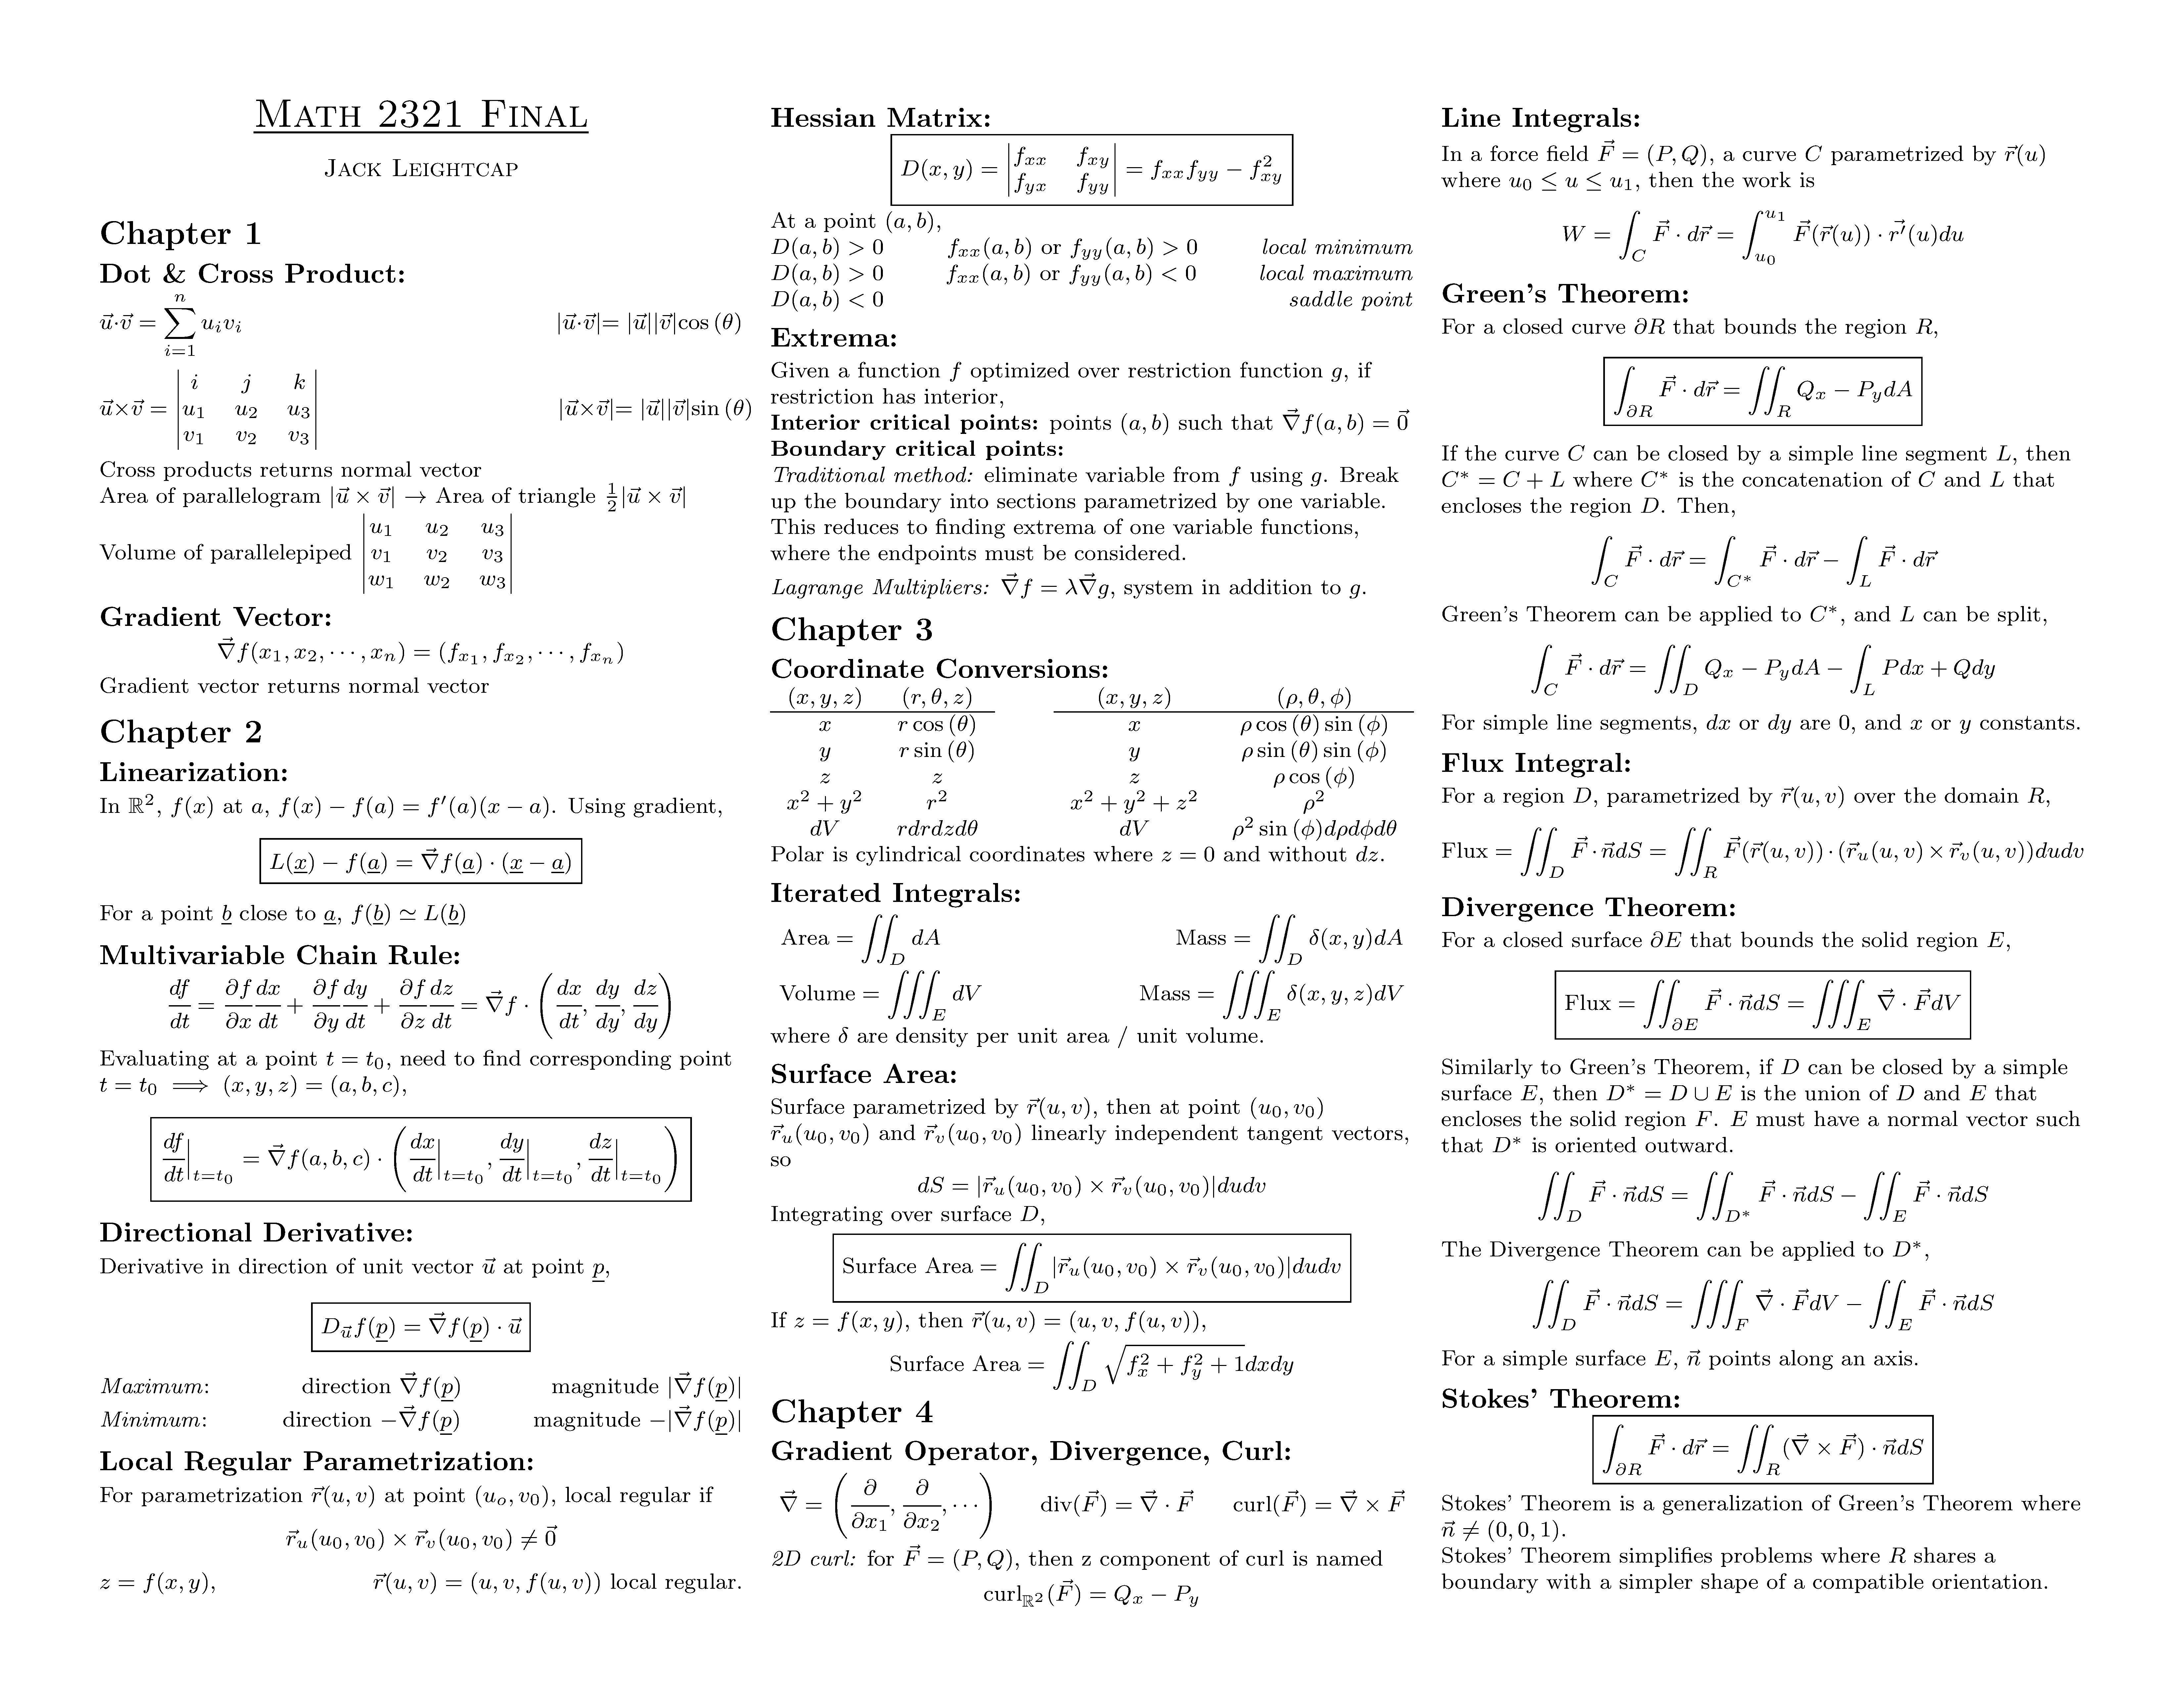
\includegraphics[height=\textheight]{CheatSheet.png}
    \vfill
\end{frame}

\begin{frame}
    \vfill
    \frametitle{How to use {\LaTeX}}
    \begin{columns}[t]
        \begin{column}{\textwidth/2}
            \begin{center}
                \textbf{Windows}
            \end{center}
            \begin{itemize}
                \item MiKTeX
                \item TeX Live
            \end{itemize}
        \end{column}
        \begin{column}{\textwidth/2}
            \begin{center}
                \textbf{Mac OS}
            \end{center}
            \begin{itemize}
                \item MacTeX
            \end{itemize}
        \end{column}
    \end{columns}
    \vfill
    \textbf{Other}
    \begin{itemize}
        \item Editors: vim and \texttt{vimtex}, emacs and \texttt{AUCTeX}
        \item IDE: VSCode and \href{https://marketplace.visualstudio.com/items?itemName=James-Yu.latex-workshop}{\texttt{LaTeX Workshop}}
        \item Online: Overleaf (what we'll be using today)
    \end{itemize}
    \vfill
\end{frame}

\begin{frame}
    \frametitle{Typesetting a Basic Document: Document Classes}
    \begin{itemize}
        \item All documents must include a \texttt{\textbackslash documentclass\{CLASS\}}.
        \item A set of defaults for specific use cases
        \item \texttt{\textbackslash documentclass[12pt, letterpaper]\{article\}}, size 12 font article
        \item \texttt{report}, longer documents, dissertation
        \item \texttt{beamer}, what made these slides
    \end{itemize}
\end{frame}

\begin{frame}
    \frametitle{Typesetting a Basic Document: Environments}
    \begin{itemize}
        \item \texttt{\textbackslash begin\{FOO\}} must be matched with \texttt{\textbackslash end\{FOO\}}, and everything between is in the \texttt{FOO} \emph{environment}.
        \item \texttt{document}: a\ldots document!
        \item \texttt{itemize}: this kind of bullet point list
        \item \texttt{center}: horizontally centered
        \item \texttt{tabular}: tables
        \item can define custom environments
    \end{itemize}
\end{frame}

\begin{frame}
    \frametitle{Typesetting Math}
    \vfill
    \begin{center}
        Time for a practical example, over to Overleaf!
    \end{center}
    \vfill
\end{frame}

\begin{frame}
    \frametitle{Helpful Tools}
    General:
    \begin{itemize}
        \item Overleaf has extensive documentation
        \item \href{http://detexify.kirelabs.org/classify.html}{Detexify} -- remembering {\LaTeX} commands is hard
    \end{itemize}
    Packages:
    \begin{itemize}
        \item \texttt{siunitx}: anything with units
        \item \texttt{circuitikz}: circuit diagrams
        \item \texttt{minted}: syntax highlighted code blocks
        \item \texttt{amsmath}, \texttt{amssymb}: extended math support
    \end{itemize}
\end{frame}

\end{document}
